\chapter {Estudis i propostes de disseny}

\section{Esquema del sistema de fitxers}

Com que volem crear una abstracci� (gen�rica) a trav�s del sistema de fitxers, a
continuaci� definirem quina ser� l'estructura de la jerarquia de fitxers i
directoris per donar suport a totes les tasques d'administraci� necess�ries
abans esmentades.

Entendrem com a '/' (arrel) l'inici de la nostra jerarquia d'administraci�.

\begin{verbatim}
/
|-- <IDCluster>
|   |-- admin
|   |   |-- 
|   |-- self
|   |   |--
|   |-- <IDNode>
|   |   |-- admin
|   |   |   |--
|   |   `-- <IDProces>
|   |       |-- 
\end{verbatim} 


\section{Soluci� cutre}
Explicaci� + figura \ref{fig:esquema-utilcl} .

\begin{figure}
   \centering
   \includegraphics[scale=0.4]{esquema-utilcl.eps}
   \caption{Esquema cutre}
   \label{fig:esquema-utilcl}
\end{figure}


\section{Soluci� guay}
Explicaci� + figura \ref{fig:esquema-supcl}.

\begin{figure}
   \centering
   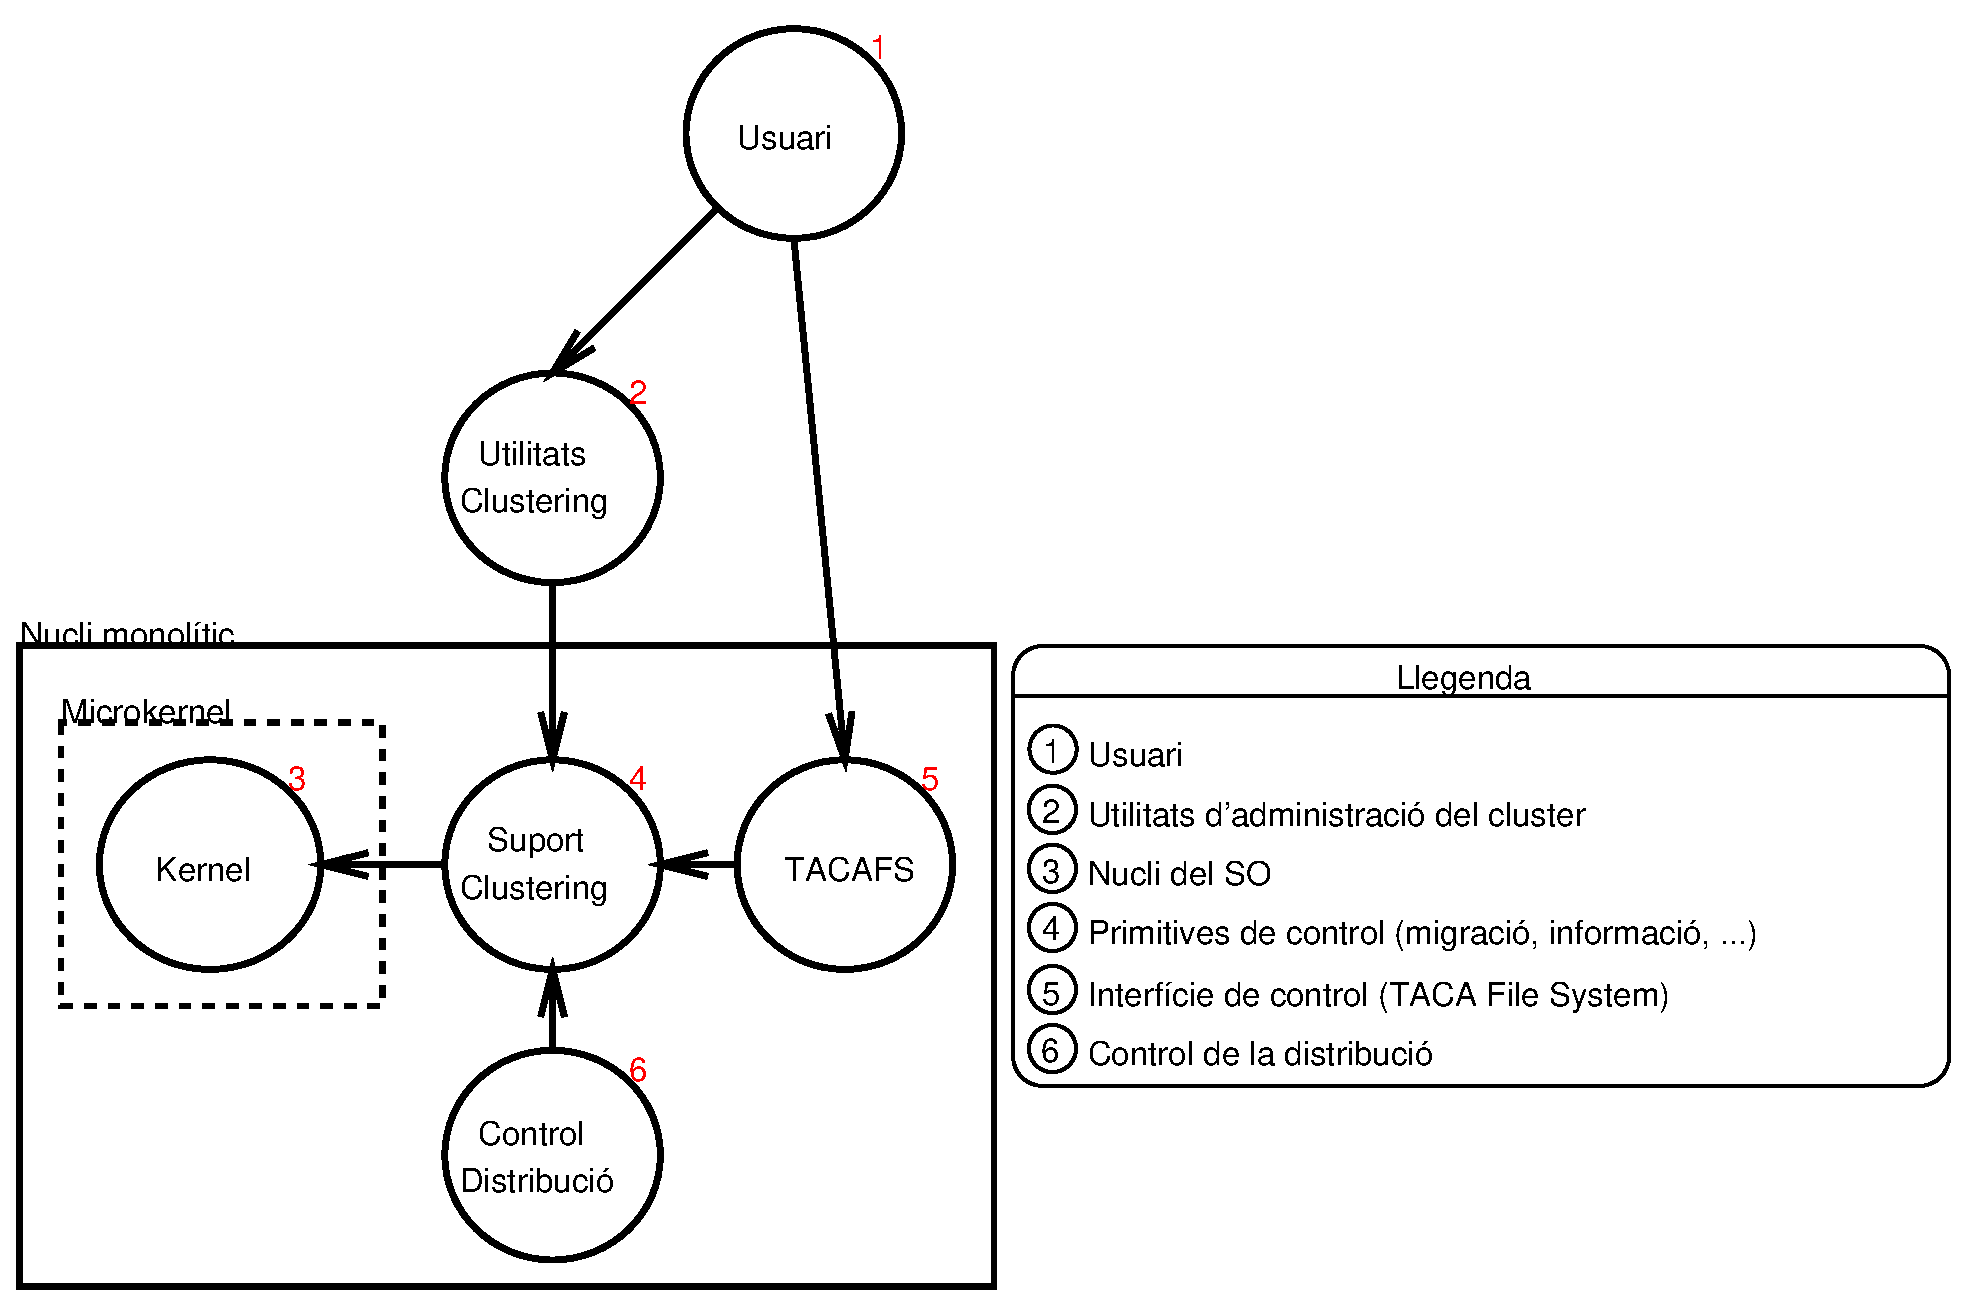
\includegraphics[scale=0.4]{esquema-supcl.eps}
   \caption{Esquema guay}
   \label{fig:esquema-supcl}
\end{figure}

\section{Soluci� super-guay}
???

\section{...}
???????


Disseny esquem�tic del sistema
==============================

Disseny a tres capes:

	Frontend	VFS
	Adaptaci�	(definici� d'una interf�cie)
	Backend		Clustering (implementaci� de la interf�cie depenent del sistema de
clustering)

Definici� d'una jerarquia:


Frontend
--------

Implementaci� de la jerarquia generica d'administraci� a trav�s de les funcions
que proporciona l'abstracci�
(sistema de fitxers virtual) del sistema sobre el que s'executa.

- Jerarquia

